\chapter{Iteration Plan 2 (FYP 1 Final)}
\label{ch:iter2}

The second iteration plan for our project is explained in this chapter. This chapter will provide guidance on the project’s modules and their development. Students are expected to talk about the project’s second stage of method of implementation in this chapter:

\section{FYP 1 Final:}
\begin{itemize}
    \item FYP 1 Final Presentation: \begin{itemize}
    \item Environment setup in Unity3D and Blender 
    \item Designed basic environment of Hospital
    \end{itemize}
\end{itemize}

\section{Designed basic environment of Hospital:}
	\begin{itemize}
	\item Reception Area
	\item Waiting Rooms
	\item Patient Rooms
	\item Training Facilities
\end{itemize}	
	
\subsection{Reception Area:}
The reception area serves as the main entrance point to the virtual hospital. It features a welcoming reception desk where virtual receptionists greet patients and visitors.
Patients can check-in here, provide necessary information.
	\begin{figure}[h]
		\centering
		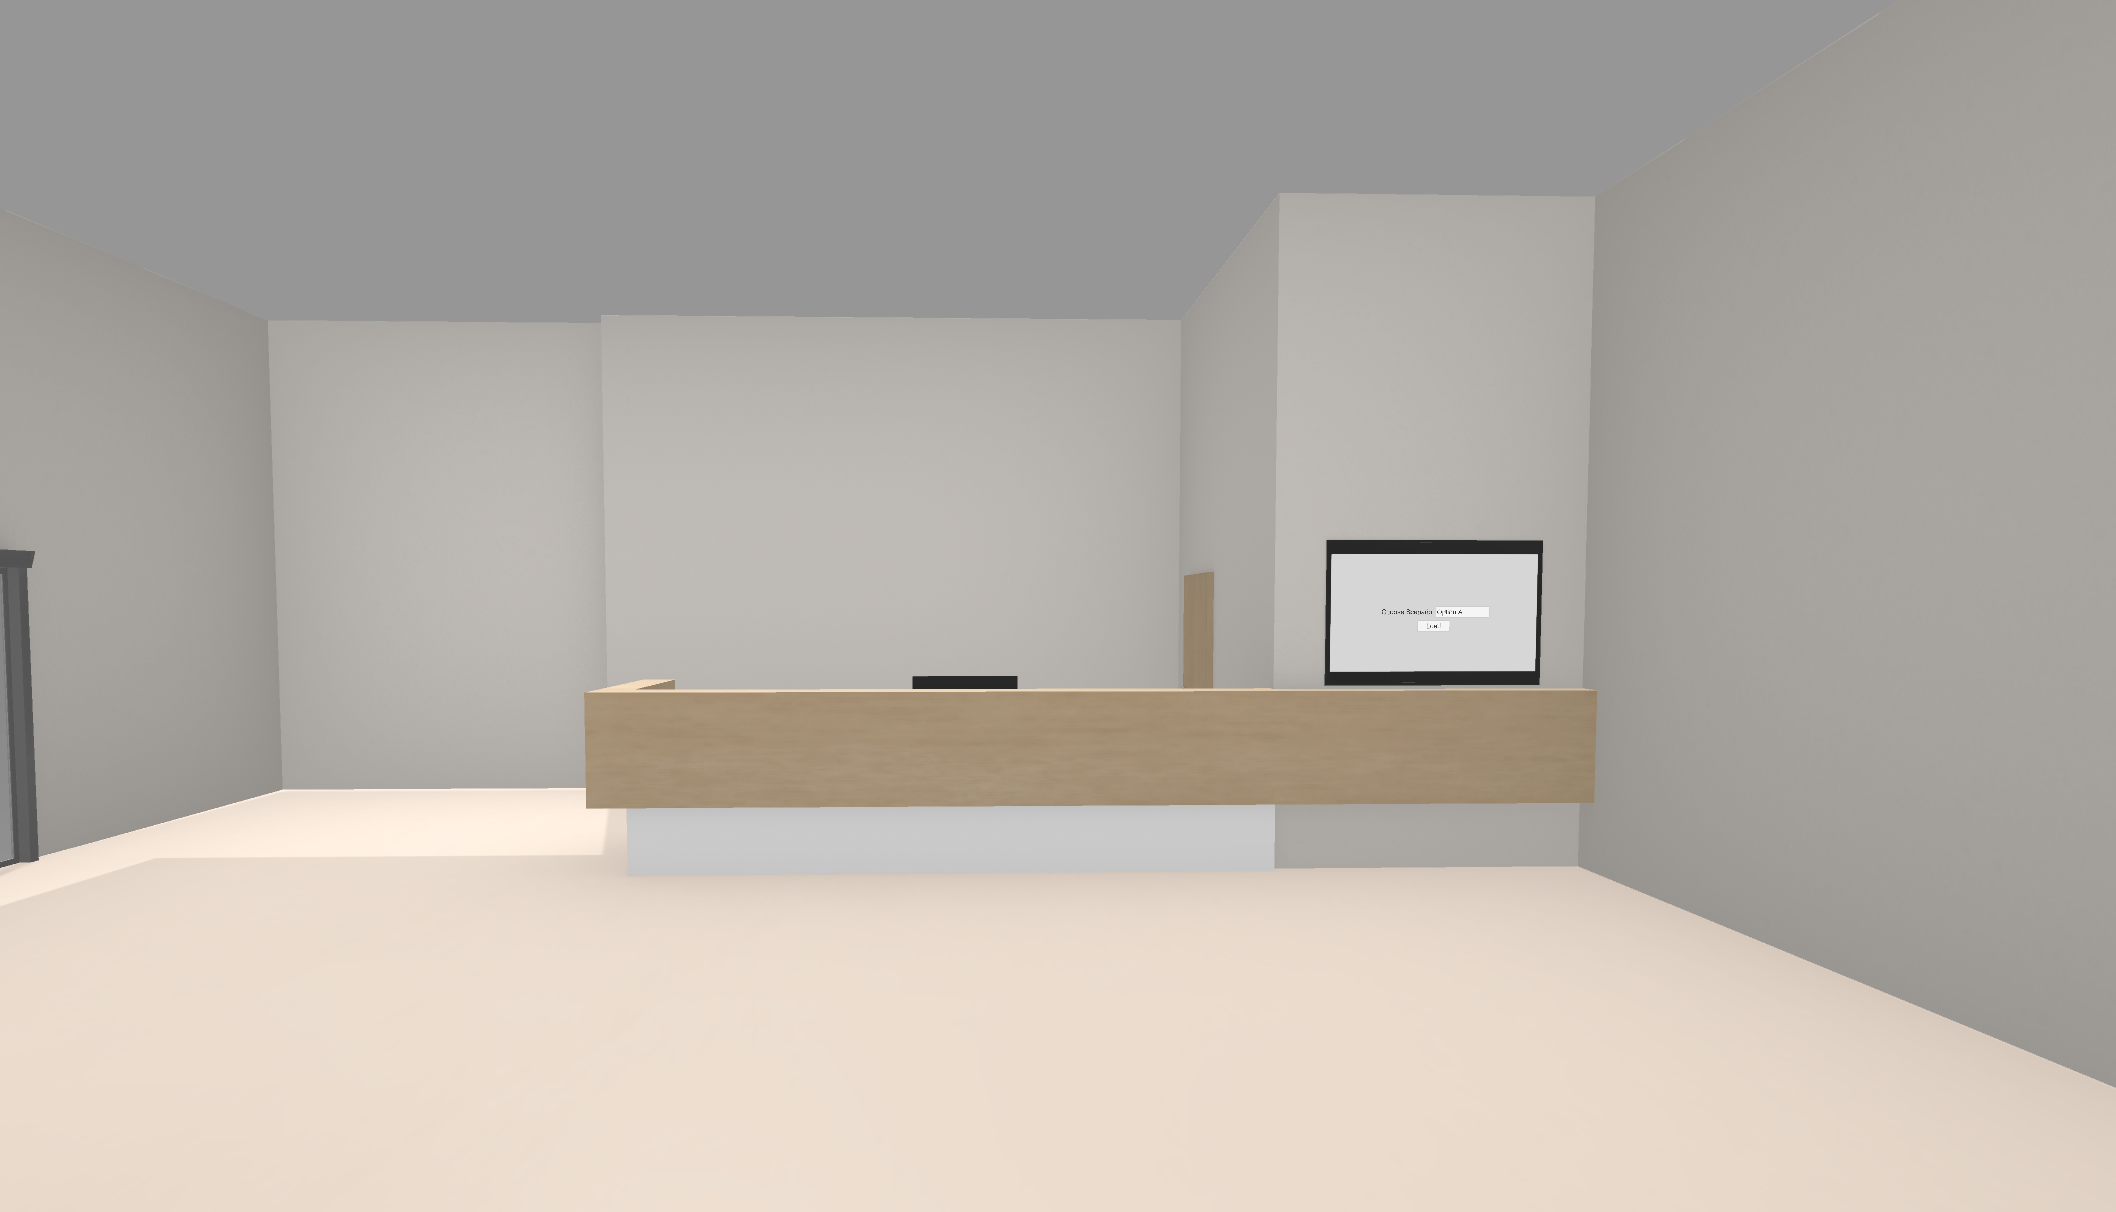
\includegraphics[width=0.7\linewidth]{Images/reception envoirnment.png}
		\caption{Reception Area}
		\label{fig:system-diagram}
	\end{figure}
\newline
\subsection{Waiting Area:}	
Waiting area is designed to mimic those found in real hospitals, providing comfortable seating arrangements for patients and their companions while they wait for appointments or procedures.
\begin{figure}[h]
		\centering
		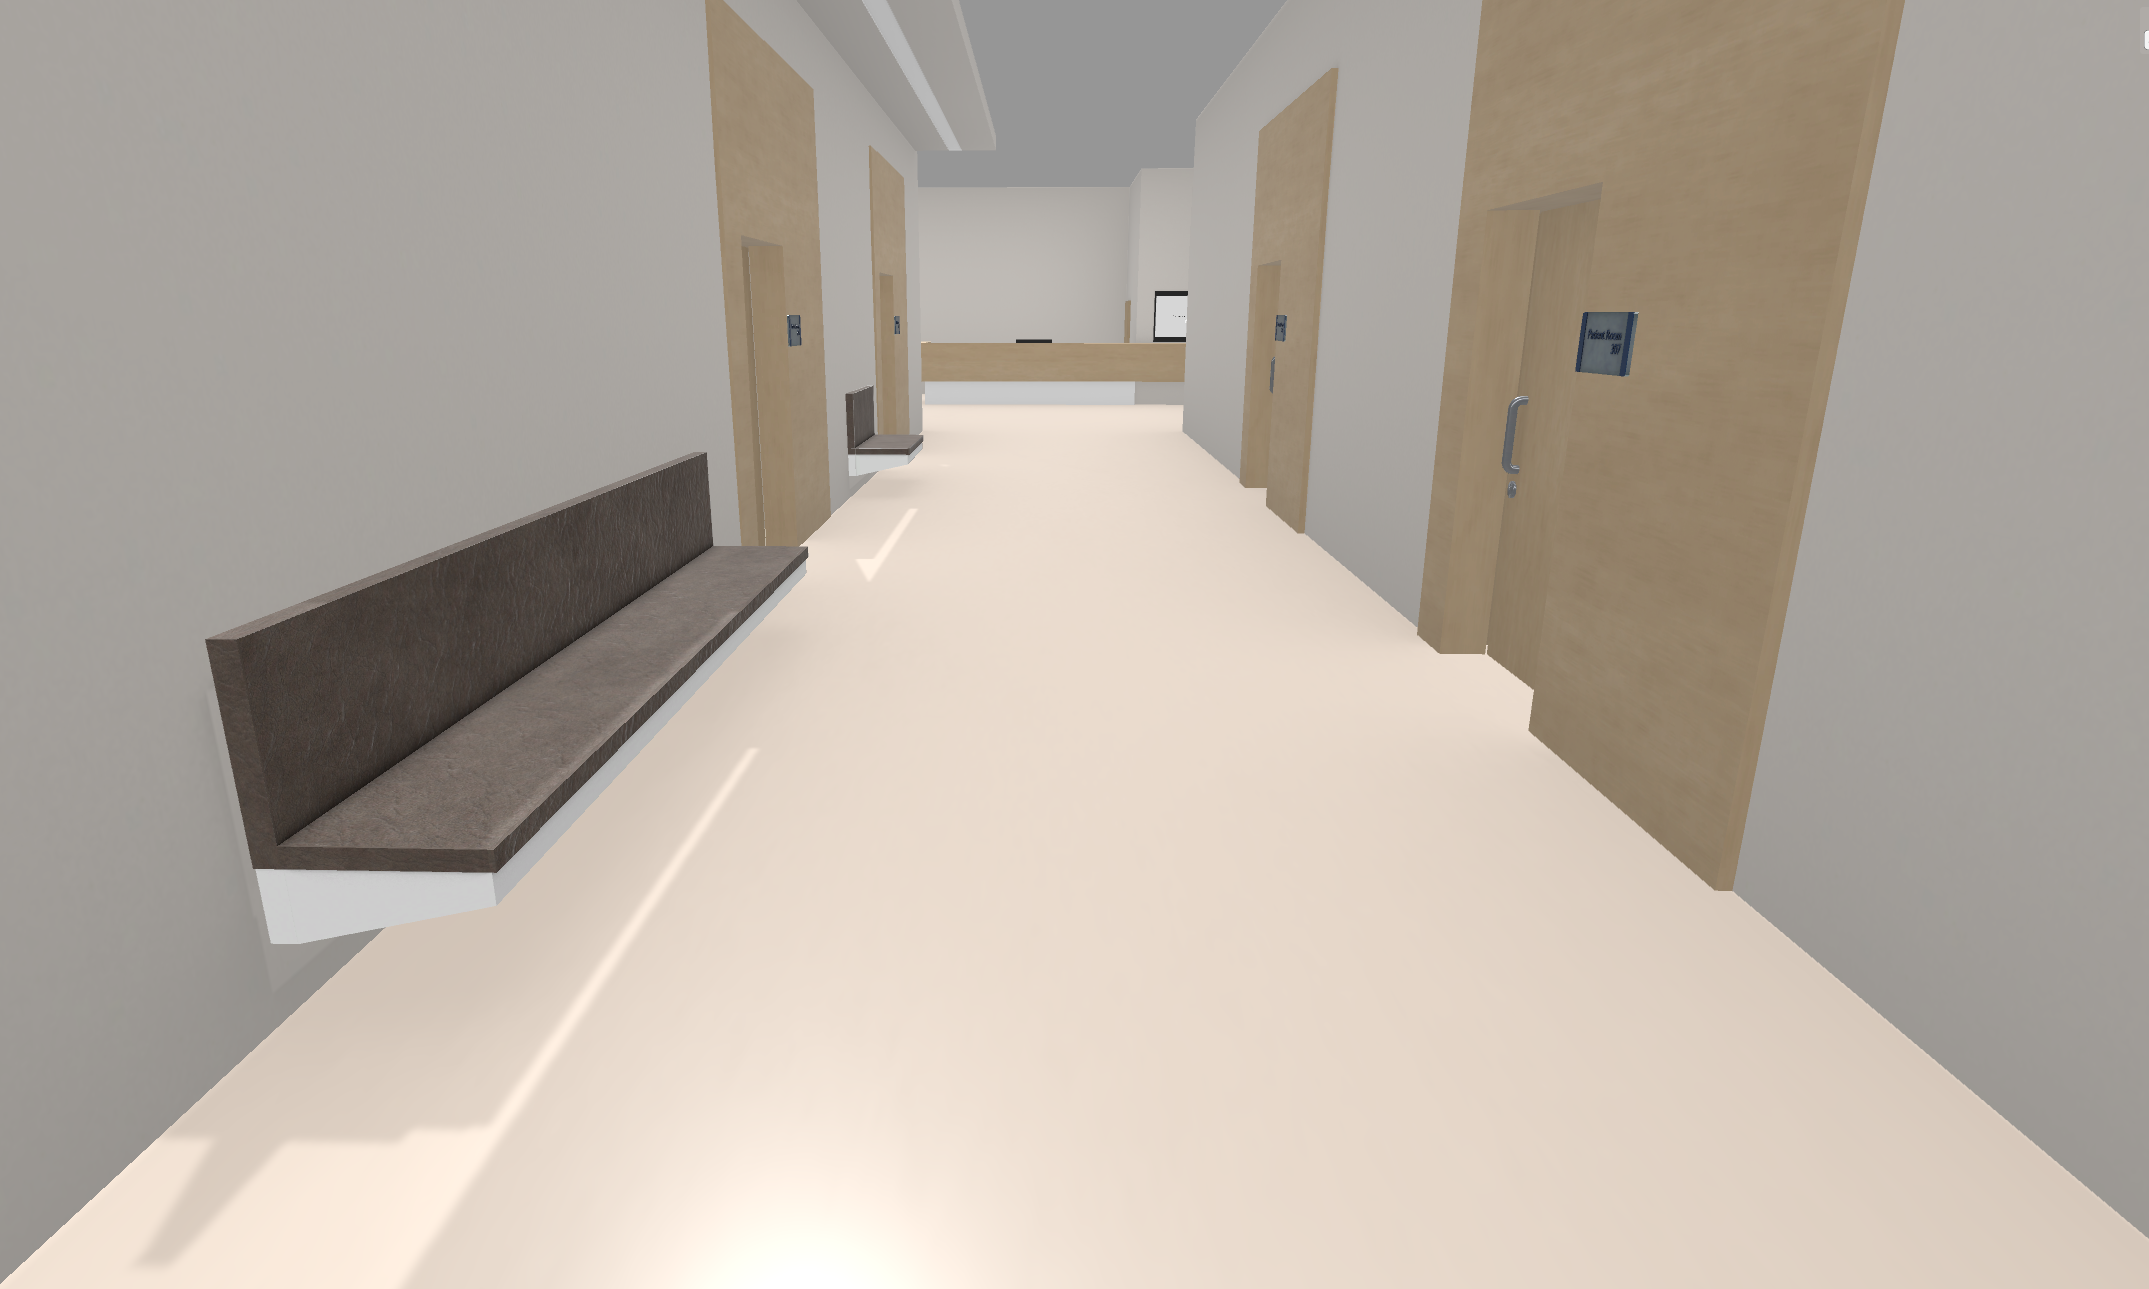
\includegraphics[width=0.7\linewidth]{Images/hospital envoirnment corridor.png}
		\caption{Waiting Area}
\end{figure}
\\
\subsection{Patient Rooms:}	
Patient rooms are designed to provide a comfortable and healing environment for patients during their hospital stay. These virtual rooms feature adjustable beds and bedside tables.
	\begin{figure}[h]
		\centering
		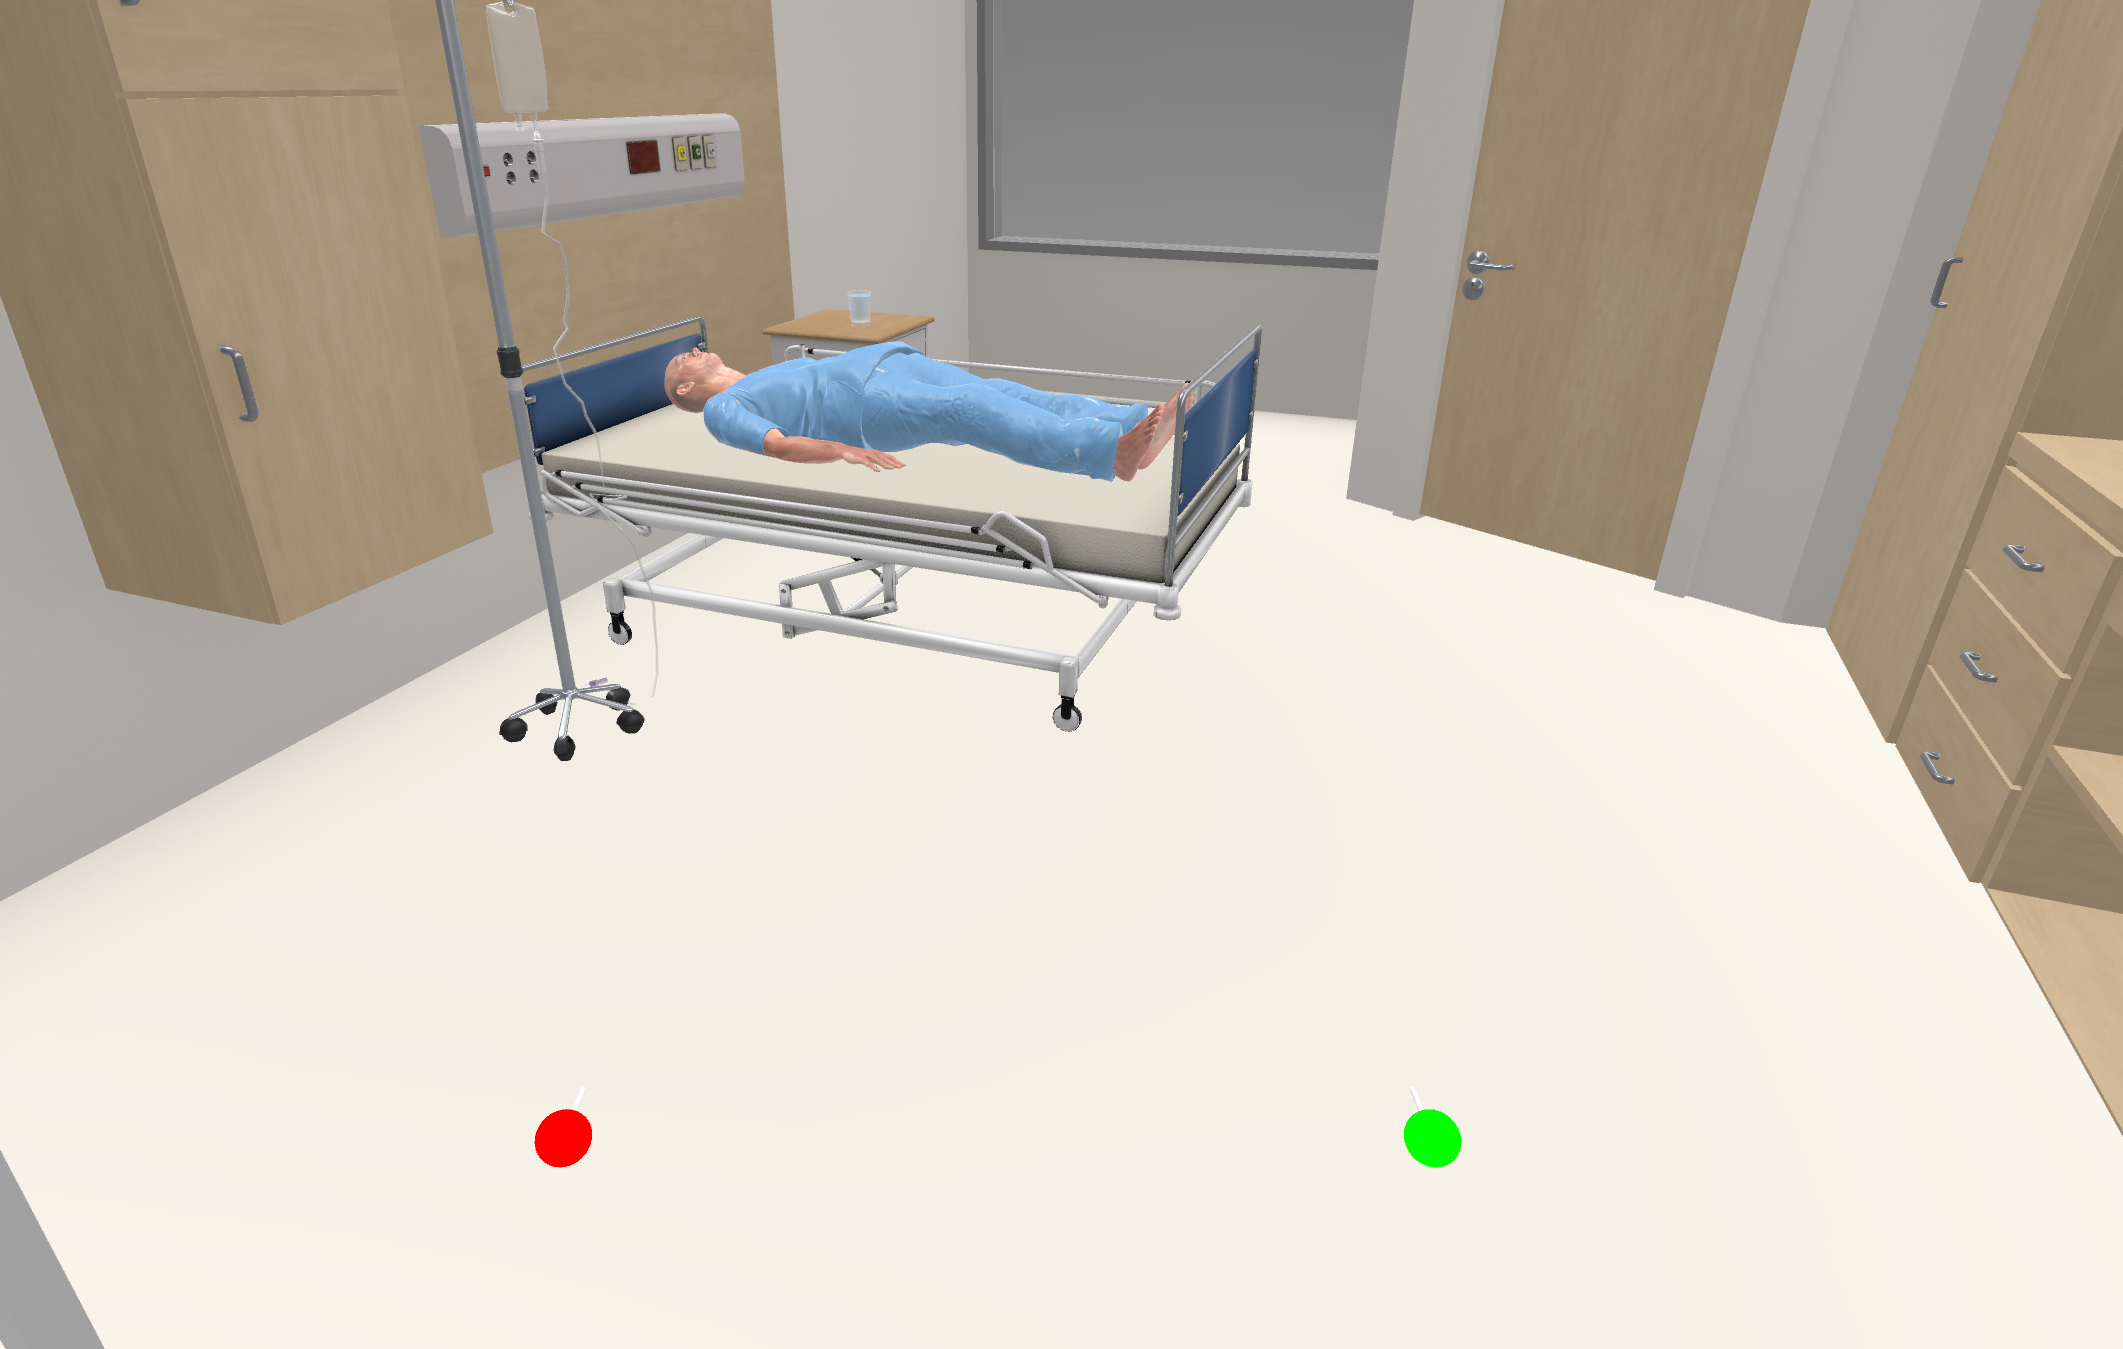
\includegraphics[width=0.7\linewidth]{Images/patient room.png}
		\caption{Patient Room}
		\label{fig:system-diagram}
	\end{figure}	

\subsection{Patient Body:}	
We created Patient Body in Metaverse Hospital to simulate patient interactions, provide realistic medical scenarios for training, and enhance learning experiences for healthcare professionals in a virtual environment.
\begin{figure}[h]
	\centering
	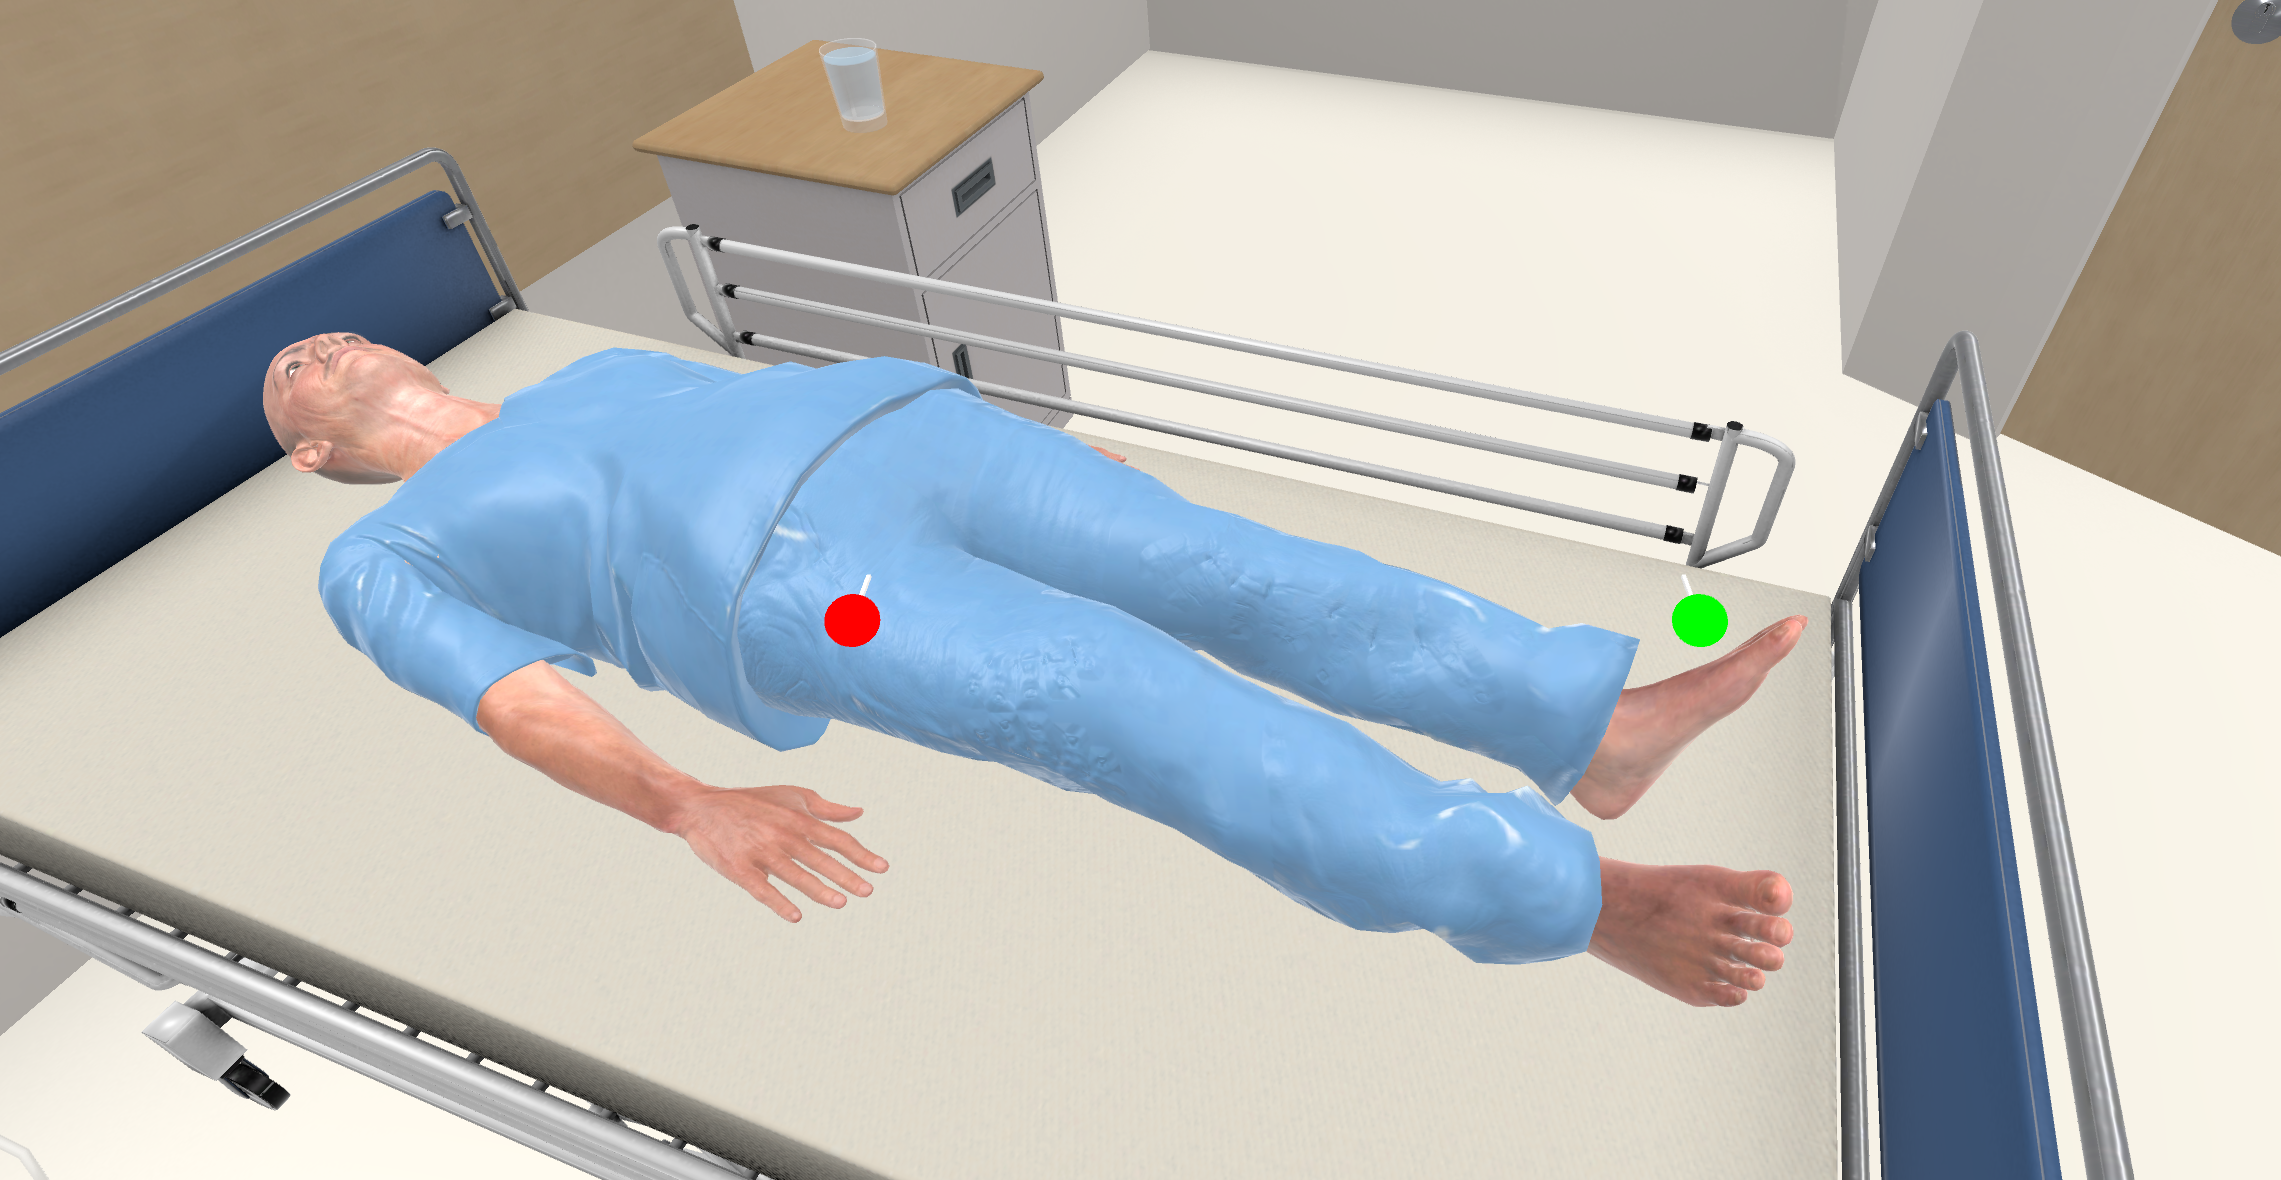
\includegraphics[width=0.7\linewidth]{Images/Patient body.png}
	\caption{Patient Room}
	\label{fig:system-diagram}
\end{figure}	

	